\documentclass[notheorems]{beamer}
\usetheme{Lab2C}
\usepackage{graphicx}
\usepackage{array}
\usepackage{subcaption}
\usepackage{listings}
\usepackage{color}
\usepackage{algorithmic}

\definecolor{mygray}{rgb}{0.5,0.5,0.5}
\lstset{
numbers=left,
numbersep=5pt,
numberstyle=\tiny\color{mygray}
}

\newif\ifbeamer
\beamertrue

\title{Ising model and its application in community detection}
\author{Feng Zhao\inst{1} \and Min Ye\inst{2}\and Shao-Lun Huang\inst{3}}
\institute{\inst{1}Dept. of Electronic Engineering, Tsinghua University
	\and \inst{2}Tsinghua-Berkeley Shenzhen Institute, Tsinghua University }
\date{December 31, 2020}
\begin{document}
\begin{frame}
	\titlepage
\end{frame}
\section*{Outline}
\begin{frame}
	\tableofcontents
\end{frame}

\section{Background}
\subsection{Ising Model}
\begin{frame}
\frametitle{Ising model}
	\begin{columns}
		\column{5cm}
		\begin{figure}
			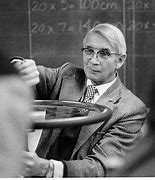
\includegraphics[width=3cm]{ernst_ising.jpeg}
			\caption{Ernst Ising, German physicist}
		\end{figure}
		\column{5cm}
	In statistical physics, Ising model refers to the magnetic spins that can be in one of two states (+1 or -1).
	
	$T_c$: critical temperature.
	
	\end{columns}
\begin{figure}
	\centering
	\begin{subfigure}{0.4\textwidth}
		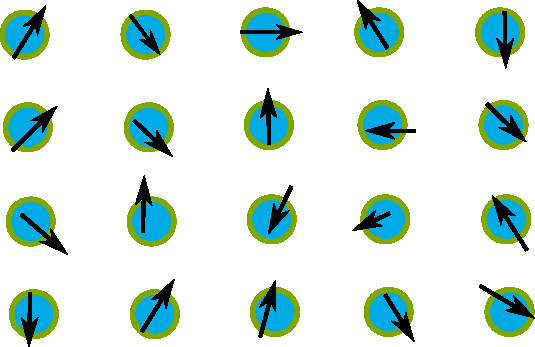
\includegraphics[width=0.7\textwidth]{Tlarge.pdf}
		\caption{$T>T_c$, random spins}
	\end{subfigure}~
	\begin{subfigure}{0.4\textwidth}
		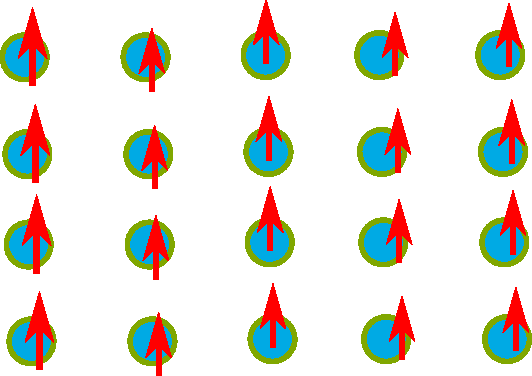
\includegraphics[width=0.65\textwidth]{Tsmall.pdf}
		\caption{$T<T_c$, spins align}
	\end{subfigure}
\end{figure}
\end{frame}
\begin{frame}
\frametitle{Canonical ensemble}
\begin{columns}
	\column{0.5\textwidth}
The distribution of particles:
\begin{equation*}
P(\sigma = \bar{\sigma}) = \frac{1}{Z} \exp(-\beta H(\bar{\sigma}))
\end{equation*}
\begin{itemize}
	\item $Z$: partition function
	\item $\beta$: inverse temperature
	\item $H$: Hamiltonian energy
	\item $\sigma \in \{\pm 1\}^n$: particle state 
\end{itemize}
	\column{0.5\textwidth}
	\begin{tabular}{ccc}
		No & Micro state & Macro state ($H$) \\
		1 & $\uparrow\uparrow\uparrow$ & -3 \\
		2 & $\uparrow\uparrow\downarrow$ & 1 \\
		3 & $\uparrow\downarrow\uparrow$ & 1 \\
		4 & $\downarrow\uparrow\uparrow$ & 1 \\
		5 & $\uparrow\downarrow\downarrow$ & 1 \\
6 & $\downarrow\uparrow\downarrow$ & 1 \\
7 & $\downarrow\downarrow\uparrow$ & 1 \\
8 & $\downarrow\downarrow\downarrow$ & -3 \\
	\end{tabular}
\end{columns}
\begin{block}{Hamiltonian for Ising model}
	Given a graph $G(V, E)$,
	\begin{equation*}
	H(\sigma) = -\sum_{\{i,j\} \in E(G)} \sigma_i \cdot \sigma_j
	\end{equation*}

\end{block}

\end{frame}
\begin{frame}
\frametitle{Square-lattice Ising model}
\begin{block}{spontaneous magnetization}
	% 磁化强度
	$M = \frac{1}{N} \sum_{i=1}^N \sigma_i$: spontaneous magnetization for $N\to \infty$:
	\begin{enumerate}
		\item $T< T_c$, $M>0$, spontaneous magnetization exists;
		\item $T> T_c$, $M=0$, no spontaneous magnetization.
	\end{enumerate}
\end{block}
\begin{figure}
	\centering
	\begin{subfigure}{0.45\textwidth}
		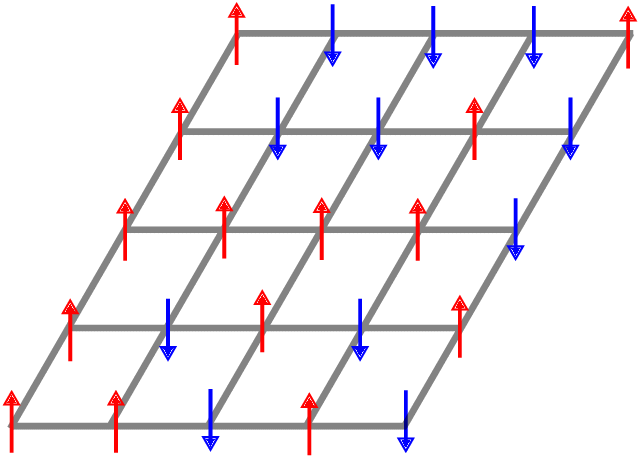
\includegraphics[width=\textwidth]{square-lattice.png}
		\caption{square lattice}
	\end{subfigure}~
	\begin{subfigure}{0.53\textwidth}
		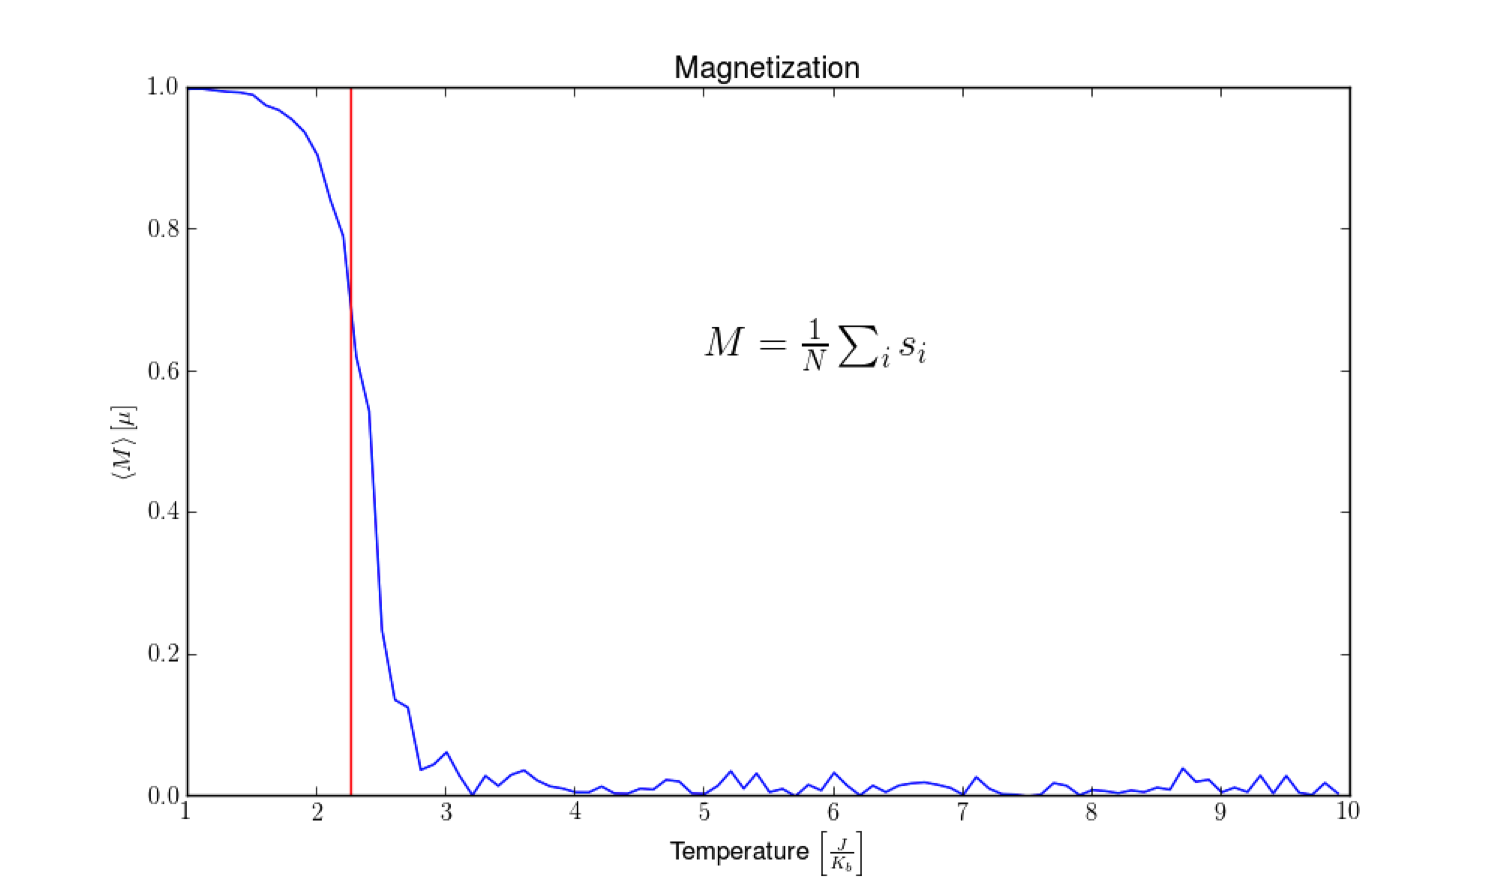
\includegraphics[width=\textwidth]{monte-carlo-ising-6.png}
		\caption{Simulation result}
	\end{subfigure}
\end{figure}

\end{frame}


\begin{frame}
\frametitle{Metropolis algorithm}
\begin{block}{Charateristics}
\begin{itemize}
	\item commonly used to simulate Ising model
	\item single-spin-flip dynamics 
	\item stochastic method for optimization
\end{itemize}
\end{block}
	\begin{algorithmic}[1]
	\STATE random initialize $\bar{\sigma}$
	\STATE randomly choosing a new state $\bar{\sigma}'$ by flipping one spin site
	\STATE compute $\Delta H= H(\bar{\sigma}') - H(\bar{\sigma})$
	\IF{$\Delta H < 0$}
	\STATE $\bar{\sigma} \leftarrow \bar{\sigma}'$
	\ELSE
	\STATE with probability $\exp(-\beta \Delta H)$ 
	such that $\bar{\sigma} \leftarrow -\bar{\sigma}'$ 
	\ENDIF
	\STATE repeat 2-8 until convergence
\end{algorithmic}
\end{frame}

\begin{frame}
\subsection{Community Detection}
\frametitle{Community detection}
\begin{columns}
	\column{0.5\textwidth}
	\begin{figure}
		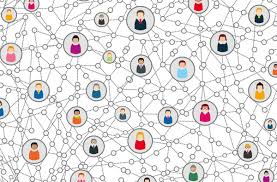
\includegraphics[width=0.8\textwidth]{cd.png}
	\end{figure}
\column{0.5\textwidth}
Community detection is inferring the group of vertices which are more
densely connected in a graph
\end{columns}
\begin{columns}
	\column{0.33\textwidth}
	\begin{figure}
		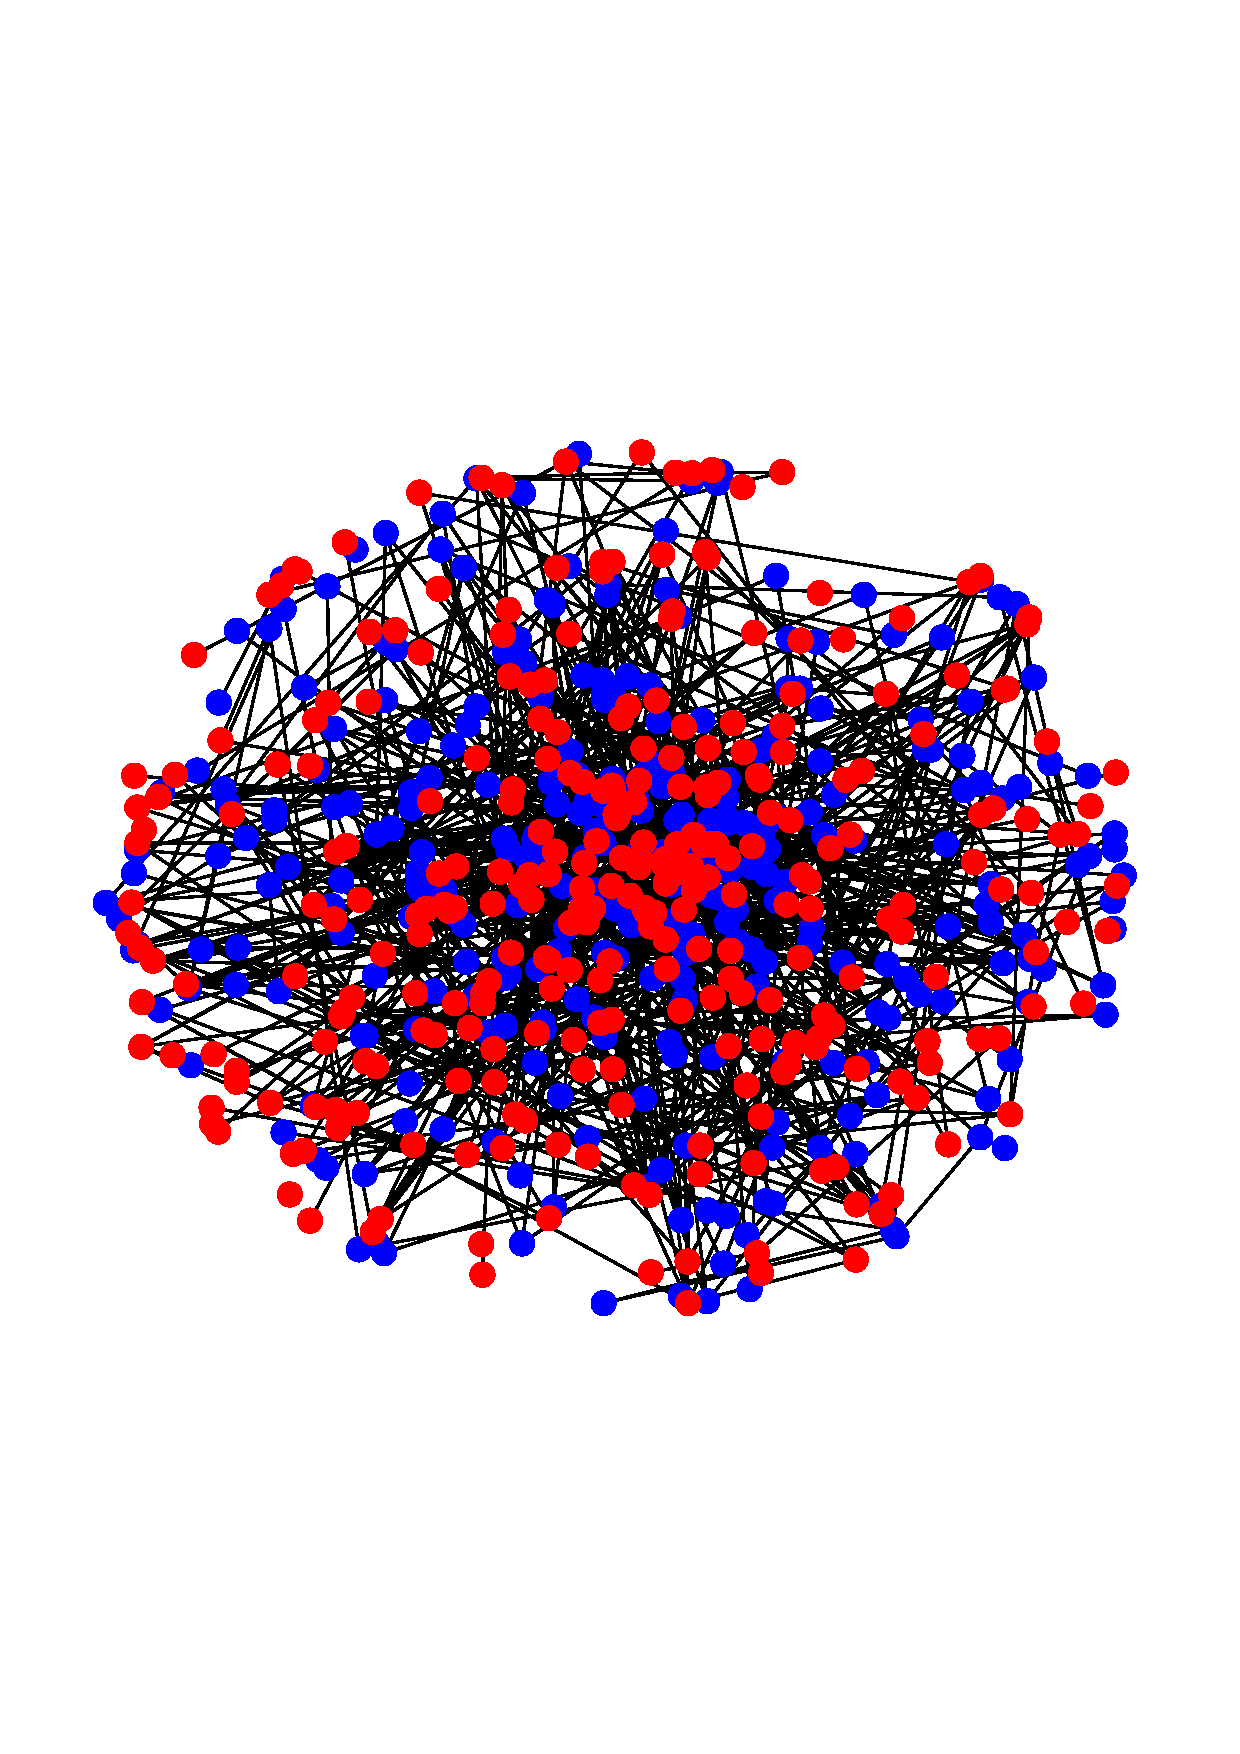
\includegraphics[width=\textwidth]{benno2t.pdf}
	\end{figure}
	\column{0.05\textwidth}
	$\Rightarrow$
	\column{0.5\textwidth}
	\begin{figure}
	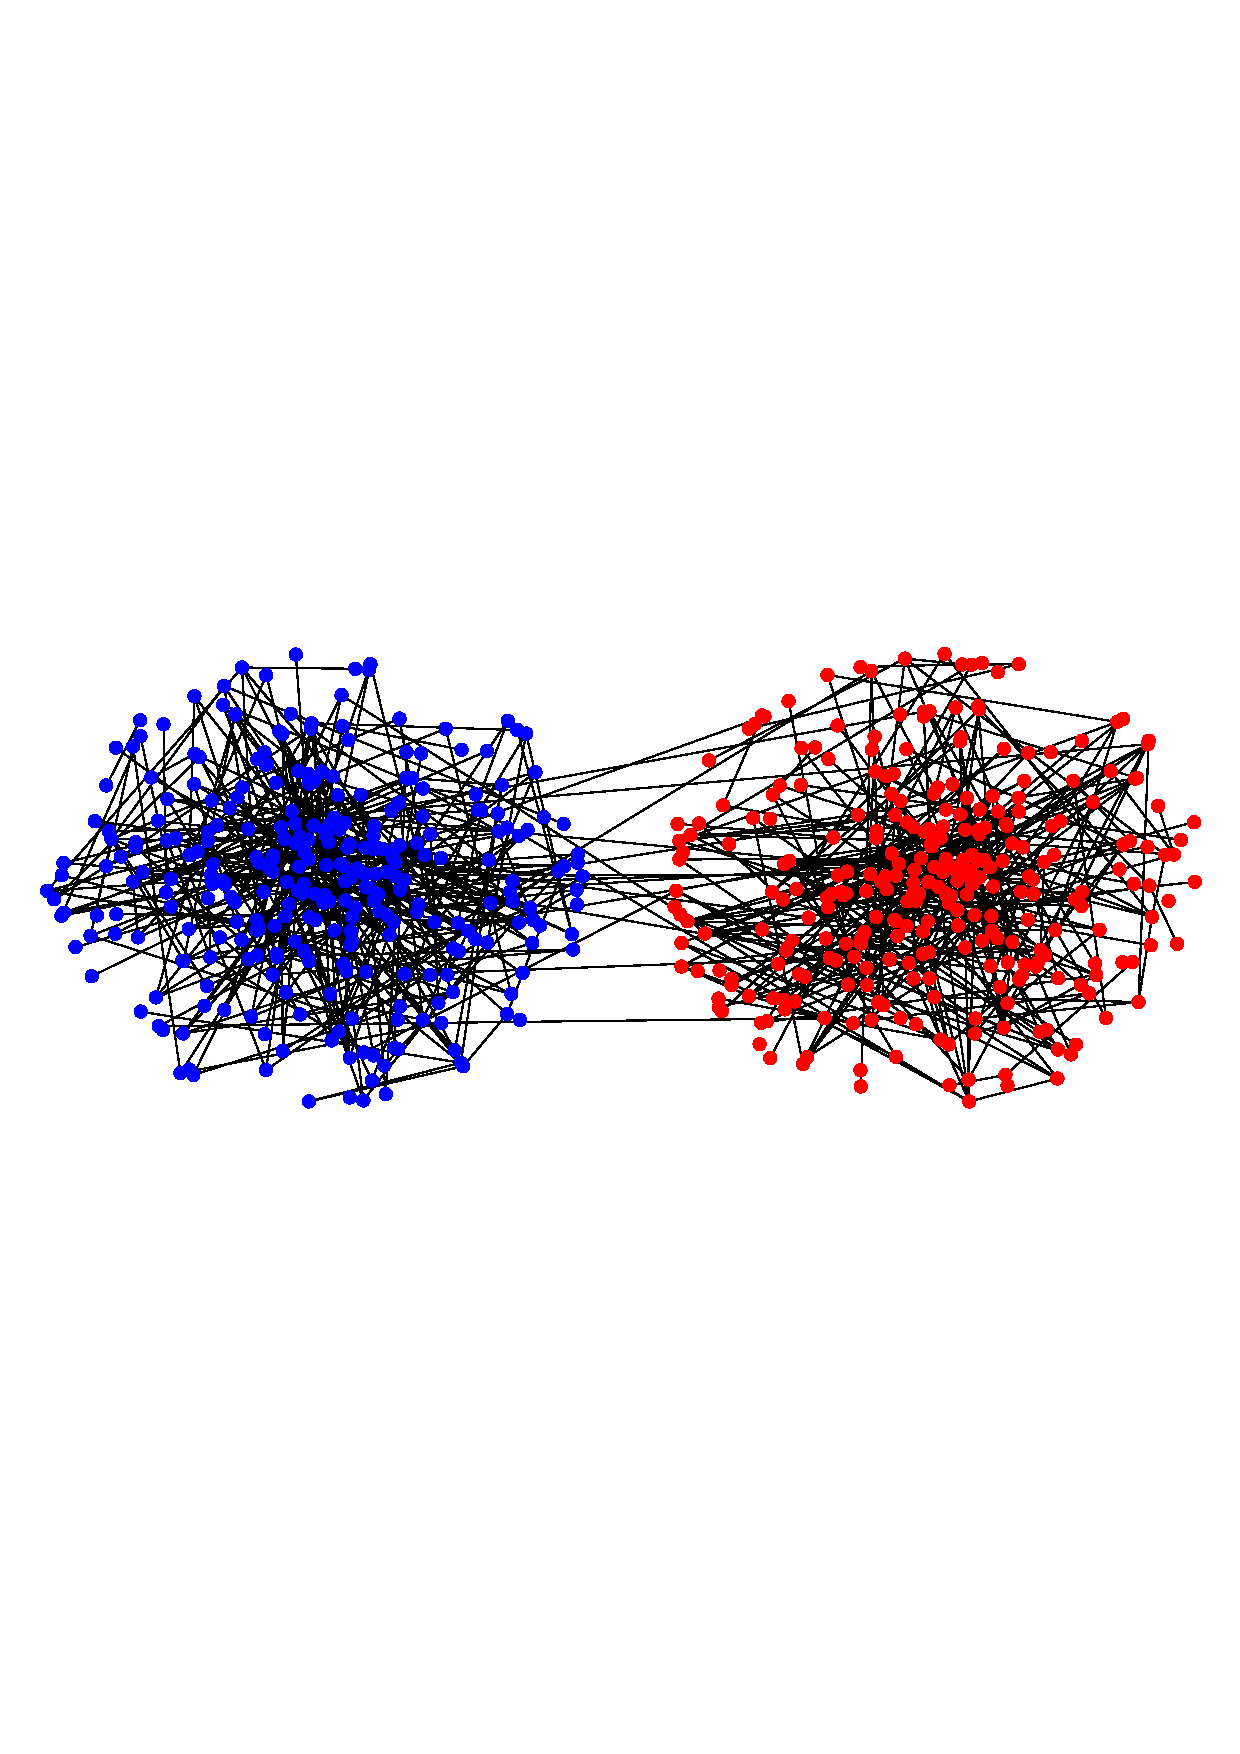
\includegraphics[width=\textwidth]{bennot.pdf}
	\end{figure}
\end{columns}


\end{frame}

\begin{frame}
\frametitle{Stochastic block model (SBM)}
\begin{block}{Characteristics}
\begin{itemize}
\item a probabilistic model to generate random graph
\item larger probability for the existence of edges within the same community
\item smaller probability for the existence of edges between different communities
\end{itemize}
\end{block}
\begin{columns}
	\column{0.33\textwidth}
		\begin{figure}
		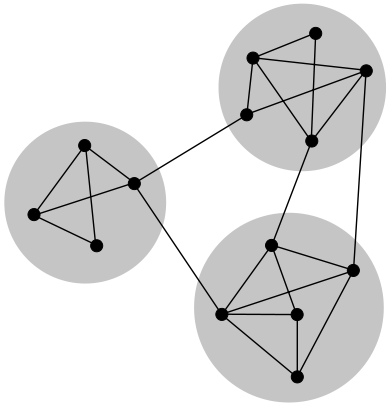
\includegraphics[width=\textwidth]{sbm.png}
	\end{figure}
\column{0.67\textwidth}
\quad$(G,X)\sim \textrm{SBM}(n, k, p, q)$
\begin{itemize}
	\item $X$: community labels
	\item $n$: the number of nodes
	\item $k$: the number of communities
	\item $p$: probability of connecting within clusters
	\item $q$: probability of connecting across clusters
\end{itemize}
\end{columns}
\end{frame}

\begin{frame}
\frametitle{Exact recovery of SBM}
\begin{description}
	\item[Observation] random graph $G$, generated by $\textrm{SBM}(n,k,p,q)$;
	\item[Estimator] $\hat{X}(G)$, an algorithm to recover node labels $X$;
	\item[Error probability] $P_e=P(\hat{X} \neq \pm X)$
\end{description}

\begin{block}{Assumptions}
	\begin{itemize}
	\item Community labels $X$ are symmetric: half $+1$, half $-1$;
	\item $p = a\frac{ \log n}{n}, q = b \frac{ \log n}{n}$;
	\item $n \to \infty$.
	\end{itemize}
\end{block}
\begin{block}{Exact recovery of SBM}
Under which condition of $a,b$ does $P_e \to 0$?
\end{block}
\end{frame}
\begin{frame}
\frametitle{Phase transition of SBM}
\begin{block}{Exact Recovery of SBM [1]}
	$P_e=P(\hat{X} \neq \pm X)$: exact recovery for $n \to \infty$
	\begin{enumerate}
		\item $\sqrt{a} - \sqrt{b} > \sqrt{2}$, $P_e \to 0$, there exists algorithms to achieve exact recovery;
		\item $\sqrt{a} - \sqrt{b} < \sqrt{2}$, $P_e \to 1$, no algorithm can achieve exact recovery
	\end{enumerate}
\end{block}
{\scriptsize [1]
Abbe, Emmanuel, Afonso S. Bandeira, and Georgina Hall. "Exact recovery in the stochastic block model." IEEE Transactions on Information Theory 62.1 (2015): 471-487.
}
\end{frame}

\section{Stochastic Ising block model}
\frame{\tableofcontents[currentsection]}
\begin{frame}
\frametitle{Stochastic Ising Block Model (SIBM)}
\begin{itemize}
\item The Ising model is defined on top of graph generated by SBM.
\begin{equation*}
P_{\sigma | G} = \frac{1}{Z} \exp(-\beta H(\bar{\sigma}))
\end{equation*}
\item The Hamiltonian energy is compensated by repelling interaction between nodes without edge connection
\begin{equation*}
H(\sigma) = \frac{p+q}{2}\sum_{\{i,j\} \not\in E(G)} \sigma_i \cdot \sigma_j - \sum_{\{i,j\} \in E(G)} \sigma_i \cdot \sigma_j
\end{equation*}
\end{itemize}
\begin{description}
	\item[Observation] random graph $G$, generated by $\textrm{SBM}(n,p,q)$;
	\item[Estimator] $\hat{X}^*$, generated by SIBM
	\item[Error Probability] $P_e=P(\hat{X} \neq \pm X) = ?$
\end{description}
\end{frame}

\begin{frame}
\frametitle{Phase transition of SIBM}
\begin{block}{Assumptions}
	\begin{itemize}
		\item Community labels $X$ are symmetric: half $+1$, half $-1$;
		\item $p = a\frac{ \log n}{n}, q = b \frac{ \log n}{n}$;
		\item $n \to \infty$.
	\end{itemize}
\end{block}
\begin{block}{Exact Recovery of SBM by $\hat{X}^*$}
	$P_e=P(\hat{X} \neq \pm X)$: exact recovery for $n \to \infty$
\begin{enumerate}
	\item $\beta > \beta^*$, $P_e \to 0$, there exists algorithms to achieve exact recovery;
	\item $\beta < \beta^*$, $P_e \to 1$, no algorithm can achieve exact recovery
\end{enumerate}
where
\begin{equation*}
\beta^* = \frac{1}{2} \log \frac{a+b-2 - \sqrt{(a+b-2)^2-4ab}}{2b}
\end{equation*}
\end{block}

\end{frame}

\begin{frame}
\frametitle{Metropolis algorithm}
Metropolis algorithm is used to approximate $\hat{X}^*$


\begin{figure}
	\centering
	\begin{subfigure}{0.45\textwidth}
		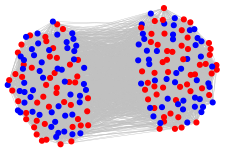
\includegraphics[width=\textwidth]{000.png}
		\caption{Initial label for $\textrm{SBM}(300, 16, 4)$}
	\end{subfigure}~
	\begin{subfigure}{0.53\textwidth}
		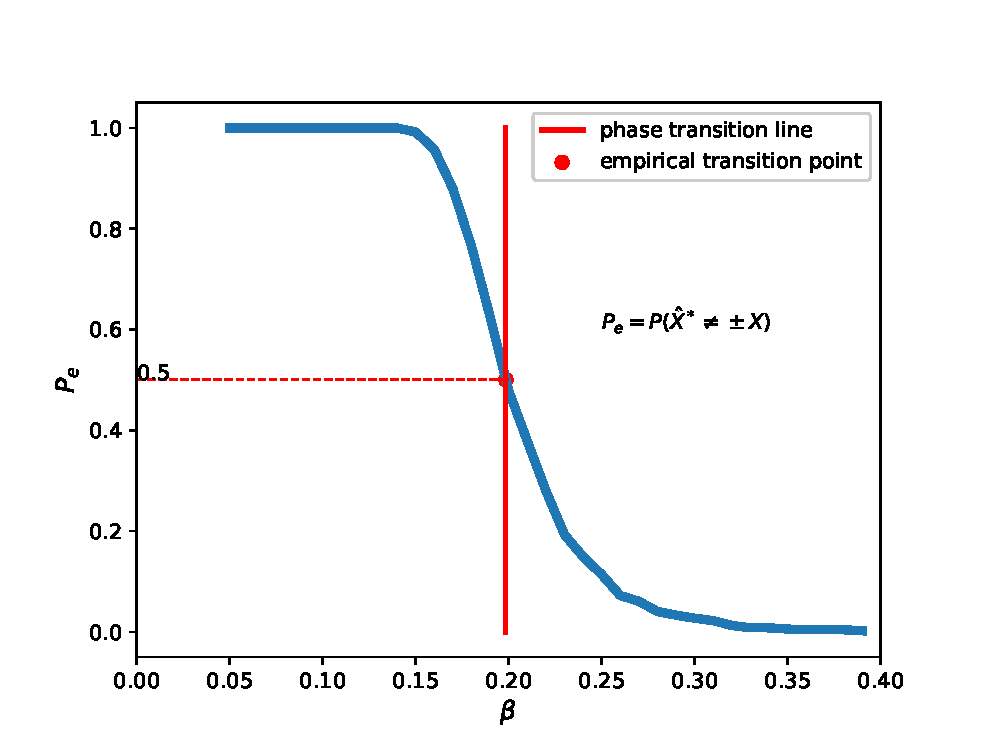
\includegraphics[width=\textwidth]{beta_trans-2020-11-28.eps}
		\caption{$\textrm{SBM}(9000, 16, 4), \beta^*=0.198$}
	\end{subfigure}
\end{figure}
\end{frame}



\section{Conclusion}
\begin{frame}
\frametitle{Conclusion}
On-going work:
\begin{itemize}
\item Extension of SIBM to multiple community case;
\item connection with other community detection method is explored
\end{itemize}
\begin{figure}
	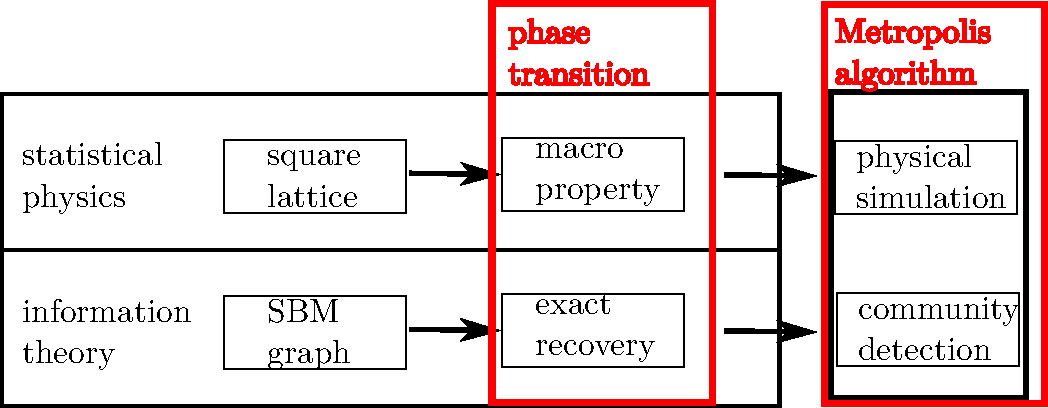
\includegraphics[width=0.8\textwidth]{overview.pdf}
	\caption{Connection between different parts}
\end{figure}
\end{frame}

\begin{frame}
\frametitle{}
\begin{block}{}
\centering
{\Huge Thank you!}
\end{block}
\end{frame}
\end{document}
